\subsection{Database Script}
\begin{figure}[htp]
\centering
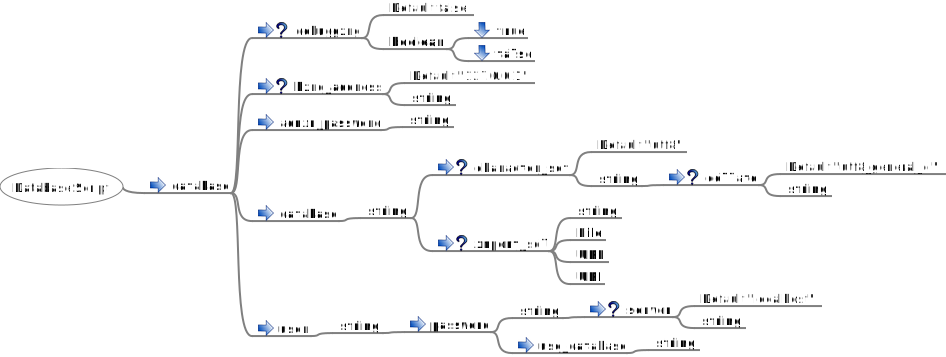
\includegraphics[width=0.9\textwidth]{database_service_script}
\label{fig:database_script_statements}
\caption{Database Script Statements}
\end{figure}


\TheStatement{database}
\TheStatement*[database]{database \{ debug bind admin database user \}}

Entry point in the database script.

\TheStatement[database:debug]{debug}
\TheStatement*[database!debug]{debug logging: \Arg{level}}

Sets the debug logging \Arg{level} for the database server. The \Arg{level}
can be any positive number, zero is normally interpreted as no logging.

\TheStatement[database:bind]{bind}
\TheStatement*[database!bind]{bind address: \Arg{address}}

Sets IP \Arg{address} or the host name on which the database server should listen
to connections. Defaults to the localhost address \qcode{127.0.0.1}.

\TheStatement[database:admin]{admin}
\TheStatement*[database!admin]{admin password: \Arg{password}}

Sets administrator \Arg{password} for the database server. If no password for
the administrator account was yet set this password is set. Used to login as
the administrator user to create users, create databases and set permissions.

\TheStatement[database:db]{database}
\TheStatement*[database!database]{database \Arg{name} [, charset: \Arg{name}] [, collate: \Arg{name}] [, \{ script \}]}

Creates a new database with the specified database \Arg{name}, character set and collate.
If the database was already on the server, it will update the character set and collate
to the specified character set and collate. The database server needs to support 
the specified character set and collate.

\TheStatement[database:script]{script}
\TheStatement*[database!script]{script execute: \Arg{resource}}

Executes the script \Arg{resource}. The resource can be a file, URL or URI. 
A string will be interpreted according to the format. If no scheme is used 
the string is assumed to be a local file.

\TheStatement[database:user]{user}
\TheStatement*[database!user]{user \Arg{name}, password: \Arg{password} [, server: \Arg{host}] [, \{ access \}]}

Creates a new user with the specified \Arg{name}, \Arg{password} and server \Arg{host}.
If the user already exists on the server, the password is updated for that user.
A user is identified by the user name and the server host.
The server host name defaults to the server host \qcode{localhost}.
The database that the user have read and write access to will be set. This will not create
the database on the server, to create a database use the \TheStatement*{database} statement.

\TheStatement[database:access]{access}
\TheStatement*[database!access]{database: \Arg{database}}

Sets the access rights for the \Arg{database} for the user. The user is granted 
all permissions to the specified database.
